\documentclass[twocolumn]{article}

\usepackage[paper=letterpaper,margin=1in]{geometry}
\usepackage{siunitx}
\usepackage{graphicx}
\usepackage{tikz}
\usetikzlibrary{circuits.ee.IEC,shapes,arrows,fit}

\title{ECEN 489: Laser Rangefinder Final Report}
\date{6 December 2013}
\author{%
  \begin{tabular}{llll}
  Clayton Crawford & Jeff Terrell   & Sam Carey    & John Boyd    \\
  Taahir Ahmed     & Ashton Jackson & Doug Maunder & Tengyan Wang
  \end{tabular}
}

\begin{document}
\maketitle

\section{Project Overview}
This project attempted to design and construct a low-cost laser rangefinder
suitable for use in robotics, safety, and mapping applications.  To measure
distance to the target, a fast signal (on the order of \SI{100}{\mega\hertz}) is
modulated on an infrared laser diode.  The light reflected off of the target
drives a phototransistor, and the reflected signal is compared to the
transmitted signal to determine the phase difference introduced by the laser
transmission path.  Separately, inertial position tracking is used to track the
movement of the emitter through space, to enable mapping of objects or
environments.  While the device produced during the project period does not work
properly, we believe that the concept is sound and could be realized over a
longer timeframe.

\section{System Breakdown}
The overall system breaks down into six modules -- three hardware and three
software.  The \emph{distance measurement} hardware module generates the
modulated beam and compares the returned signal to the transmitted signal to
perform distance determination.  The \emph{beam scanner} uses an angled mirror
on a motor with coupled encoder to sweep the beam in a plane and report the
current beam angle to the user.  The \emph{inertial measurement unit} uses an
integrated circuit accelerometer and gyroscope to report linear and angular
acceleration to the software pipeline.  On the software side, the \emph{pose
  integrator} takes the reported accelerations and produces the current 3D pose
of the device.  The \emph{pose transformation} module takes the reported ranges
and angles and produces measurement points in the reference frame produced by
the pose integrator.  Finally, the \emph{visualizer} displays the points using
OpenGL.  Figure \ref{fig:project-block-diagram} shows the overall information
flow between the project modules.

The microcontroller used to coordinate the hardware modules and communicate with
the attached computer is an Atmel AT90USB1286, chosen for its high clock rate
and built-in USB stack.  Direct USB communication has several advantages over
the typical USB-serial or serial communication, the most compelling of which is
the ability for the device to uniquely identify itself using vendor and device
ids that are recognized by a driver on the computer.  In addition, the USB
specification has an add-on specification (a USB \emph{class}) called the USB
Test and Measurement Class, which defines message formats for generic
USB-attached measurement equipment; the Linux kernel has a built-in
understanding of Test and Measurement devices, allowing the rangefinder to be
identified and used with little effort.

\begin{figure}[h]
  \centering
  \small
  
% Needs shapes, arrows, and fit libraries.

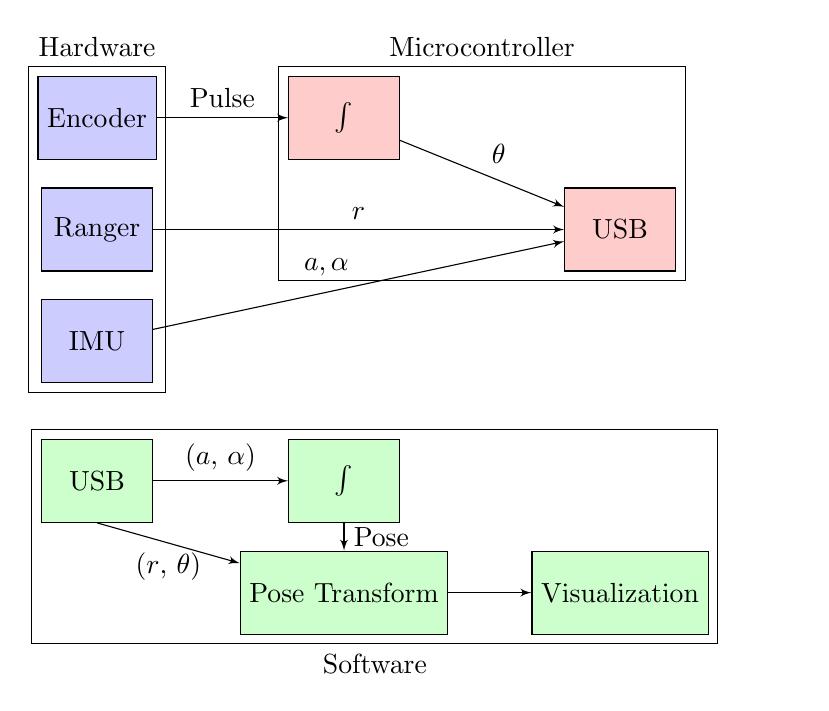
\begin{tikzpicture}[auto, node distance=3cm, >=latex']

% sensor style
\tikzstyle{sn} = [
    draw,
    fill=blue!20,
    rectangle,
    minimum height=3em,
    minimum width=4em
]

% microcontroller style
\tikzstyle{uc} = [
    draw,
    fill = red!20,
    rectangle,
    minimum height=3em,
    minimum width=4em
];

% PC Style
\tikzstyle{pc} = [
    draw,
    fill = green!20,
    rectangle,
    minimum height = 3em,
    minimum width = 4em
]

% Place the nodes.
\matrix [row sep = 1em, column sep = 3em]
{
    \node [sn] (encoder) {Encoder};
    & \node [uc] (enc-int) {$\int$};
    &                         
    \\
    
    \node [sn] (ranger) {Ranger};
    &
    & \node [uc] (usb) {USB};
    & 
    \\
    
    \node [sn] (imu) {IMU};
    &
    &
    \\

    &&&\\

    \node [pc] (pc-usb) {USB};
    & \node [pc] (imu-int) {$\int$};
    &                         
    \\

    % Nothing in first cell.
    & \node [pc] (pose) {Pose Transform};
    & \node [pc] (viz) {Visualization};
    &
    \\ 
};

% Connect the nodes.
\draw [->] (encoder) -- node {Pulse} (enc-int);
\draw [->] (ranger) -- node {$r$} (usb);
\draw [->] (imu) -- node {$a, \alpha$} (usb);
\draw [->] (enc-int) -- node {$\theta$} (usb);
\draw [->] (imu-int) -- node {Pose} (pose);
%\draw [->] (tuple) -- node {To PC} (exit);

\draw [->] (pc-usb) -- node {($a$, $\alpha$)} (imu-int);
\draw [->] (pc-usb.south) -- node [below] {($r$, $\theta$)} (pose);
\draw [->] (pose) -- (viz);

% Draw fitting boxes.
\node[draw, fit= (encoder) (ranger) (imu), label=above:{Hardware}] {};
\node[draw, fit= (enc-int)  (usb), label=above:{Microcontroller}] {};
\node[draw, fit= (pose) (viz) (imu-int) (pc-usb), label=below:{Software}] {};

\end{tikzpicture}

  \caption{Module representation of the project, with information flow
    indicated.}
  \label{fig:project-block-diagram}
\end{figure}

\subsection{Hardware -- Ranger}

\emph{Jeff Terrell, John Boyd, Taahir Ahmed, Doug Maunder}

The heart of the range measurement module is the AD8302 phase/gain measurement
chip.  On the device, we have a high frequency oscillator that drives an
infrared laser diode.  This modulated light beam travels out to its target and
bounces back to a phototransistor mounted coaxially with the laser diode.  The
phase difference between the transmitted and received signal is proportional to
the path length of the laser, with a small constant offset introduced by the
amplification circuitry.  The microcontroller takes the phase measurement from
the AD8302 and scales it according to its calibration to produce a range. A
block schematic of our range detection circuit is shown in Figure
\ref{fig:ranger-block}.

\begin{figure}[h]
  \centering
  \includegraphics[width=\columnwidth]{ranger-block}
  \caption{Block diagram of the ranger circuitry.  The current drive block is
    not an integrated circuit; rather, it is a custom drive circuit.}
  \label{fig:ranger-block}
\end{figure}

\subsection{Hardware -- Inertial Measurement Unit}

\emph{Ashton Jackson, Sam Carey}

The IMU’s accelerometer records coordinate points in an egocentric frame. The
gyroscope reads units in degrees per second, and the accelerometer reads them in
g. First, the I2C communication is initialized, and the accelerometer is set to
measure mode with a range of +/- 4G and scaled accordingly. The I2C clock speed
is set at 50 kHz. As the most recent Euler’s angles (roll, pitch, and yaw) are
read, they are stored in x, y, and z variables. This occurs in an infinite loop
with a delay of 100 microseconds. The microcontroller then transfers the angles
from the hardware’s egocentric frame to a common world frame.

\subsection{Hardware -- Beam Director}

\emph{Sam Carey, Doug Maunder}

The laser diode and phototransistor are installed parallel to each other on the
mainboard, pointing forward. They look into a two-inch mirror angled at 45
degrees and mounted on the tip of a motor shaft pointing back coaxially at the
mainboard. A 3D-printed frame holds the motor in this position by a thin
armature. The 3D-printer was also used to mount the mirror to the motor
shaft. As the motor shaft and mirror rotate, the laser beam’s reflection is
redirected at a constant angular frequency, circularly scanning a plane
perpendicular to the shaft and the fixed beam from the mainboard. As the laser
sweeps across various surfaces in the environment, its backscatter is detected
through the mirror by the phototransistor. A small slice of the plane is
obscured from the laser’s scan by the motor’s supporting armature. Taking
advantage of this, the blocking effect triggers a reset in the beam’s present
angle counter, thereby calibrating the starting angle relative to the
mainboard. Intermediate angles, between armature scans, are tracked by the
motor’s built-in encoder.

\subsection{Software -- Pose Integration}

\emph{Taahir Ahmed}

The pose integrator takes linear and angular acceleration data from the IMU and
produces a 3D pose for use by the pose transformation unit.  Each integration
step is modeled as an instantaneous rotation due to the angular acceleration,
followed by a linear offset from the linear acceleration.  This is a common
spatial integration strategy that produces accurate results provided the
underlying integration scheme is accurate and updates are closely spaced.  There
are two separate integration schemes used. The angular integration is handled by
a Lie group integration scheme in which angular acceleration, velocity, and
position are modeled as unit quaternions.  A Lie group integration scheme (as
opposed to simple Euler or even Runge-Kutta integration) respects the
unit-length constraint on the quaternions, giving a very accurate integration.
The linear integration is handled by a standard runge-Kutta scheme using batched
updates.

After integration, the pose consists of a unit quaternion (orientation) and a
3-vector (position).  This representation is converted to a 4-by-4 affine
transform matrix for use in the pose transformation stage.

\subsection{Software -- Pose Transformation}

\emph{Clayton Crawford, Tengyan Wang}

This module takes the current pose from the pose integrator and uses it to
transform measurements from the rangefinder and beam director from the
hardware's egocentric reference frame to a common world frame for display.  The
overall world-frame result is given by
\begin{equation}
  p_w = A B p_e,
\end{equation}
where A is the affine transform matrix produced by the pose integrator, B is the
affine transform matrix that represents the angle recorded by the beam director,
and $p_e$ is the egocentric range vector $[r\ 0\ 0\ 1]^T$.  In order to construct
the matrices and perform matrix operations, the Armadillo linear algebra library
is used. The JSONcpp library is used to send the resulting data, after matrix
multiplication, to the visualization stage.

\subsection{Software -- Visualization}

\emph{Tengyan Wang, Clayton Crawford}

The visualization receives the data set after pose transformation and then uses
these data for OpenGL display. Original data are sets of 3D point with x,y,z
variables collected by IMU, pose transformation transforms the data from their
local coordinate systems to a global coordinate system. Since all the points are
in the same coordinate system, they can be directly displayed using OpenGL
functions. We are using freeglut3 library and include 'glut.h' in our
visualization program. The typical OpenGL display uses the form
glutDisplayFunc(function) in the main function, the 'function' within
parentheses is used for plotting 3D points in the display window. Besides
display function, other functions like rotation, zoom in/zoom out viewing and
change viewing point are applied, all of these functions involves real-time 3D
motion.

The test part of visualization is based on random or manipulated data with Json
output and input. The input data are generated by a test program, which can
write random/manipulated data in the form of Json object to a certain file,
acting like it's the data received from pose transformation. Then the
visualization program also creates the same form of Json object and read Json
from input file, at last displays 3D points with x,y,z variables. An example
simulated scan of a pipe with a deformity is shown in Figure
\ref{fig:simulated-pipe-deformity}.

\begin{figure}
  \centering
  \includegraphics[width=\columnwidth]{simulated-pipe-deformity}
  \caption{Output of pose transformation and visualization pipeline for
    simulated data of a pipe with a circular deformity.}
  \label{fig:simulated-pipe-deformity}
\end{figure}

\section{System Status}

At the end of the project period, the rangefinder system is incomplete.  The
software pipeline is completed and tested (with the exception of the pose
integrator), as well as the IMU and beam director.  The primary defect is in the
rangefinder unit; specifically, the modulation driver circuitry.  The current
design uses an op-amp to directly drive the laser diode.  However, the slew rate
required in this configuration is beyond the capability of any reasonably-priced
op-amp.  To fix this, the circuit shown in Figure \ref{fig:current-sense-driver}
is proposed.  It uses the op-amp in an inverting configuration to drive the gate
of a MOSFET.  The MOSFET then drives the laser diode in a current-drive
configuration.  Instead of directly trimming to its output, the op-amp trims to
the voltage across a small current-sense resistor, which ensures that the
current through (and the power emitted by) the laser diode follows the
modulation function well.

\begin{figure}[h]
  \centering
  
% Needs circuit library.



\begin{tikzpicture}[circuit ee IEC, tiny circuit symbols]

  % The PGF macros below use the plain-TeX convention of the at-sign in command
  % names.
  \makeatletter
                            
  % Declare an NPN mosfet shape.
  \pgfdeclareshape{npn-mosfet-basic-shape}
  {
    \savedanchor{\centerpoint}{%
      \pgfpoint{0}{0}%
    }

    \anchor{center}{%
      \centerpoint%
    }

    \anchor{gate}{%
      \pgfpointadd{\centerpoint}{\pgfpointxy{-0.5}{0}}%
    }

    \anchor{drain}{%
      \pgfpointadd{\centerpoint}{\pgfpointxy{0}{0.2}}%
    }

    \anchor{source}{%
      \pgfpointadd{\centerpoint}{\pgfpointxy{0}{-0.2}}%
    }

    \anchor{input}{%
        \pgfpointadd{\centerpoint}{\pgfpointxy{0}{0.2}}%
    }

    \anchor{output}{%
        \pgfpointadd{\centerpoint}{\pgfpointxy{0}{-0.2}}%
    }

    \backgroundpath{%

      % Move to the start of the gate line.
      \pgfpathmoveto{\pgfpointxy{-0.5}{0}}
      \pgfpathlineto{\pgfpointxy{-0.27}{0}}

      \pgfpathmoveto{\pgfpointxy{-0.27}{0.17}}
      \pgfpathlineto{\pgfpointxy{-0.27}{-0.17}}
      
      \pgfsetarrowsend{latex}
      \pgfpathmoveto{\pgfpointxy{0}{0.2}}
      \pgfpathlineto{\pgfpointxy{-0.22}{0.2}}
      \pgfpathlineto{\pgfpointxy{-0.22}{-0.2}}
      \pgfpathlineto{\pgfpointxy{0}{-0.2}}
    }
  }

  % Declare a "voltage bar" shape.
  \pgfdeclareshape{voltage-bar-shape}
  {
    \savedanchor{\centerpoint}{
      \pgfpointxy{0}{0}
    }
 
    \anchor{center}{%
      \centerpoint
    }

    \anchor{output}{%
      \centerpoint
    }
    
    \anchor{input}{%
      \pgfpointxy{0}{0.05}
    }
 
    \backgroundpath{
      \pgfpathmoveto{\pgfpointxy{-0.2}{0}}
      \pgfpathlineto{\pgfpointxy{0.2}{0}}
    }
  }

  % Declare an op-amp, inverting input below.
  \pgfdeclareshape{op-amp-neg-down-shape}{

    \savedanchor{\centerpoint}{
      \pgfpointxy{0}{0}
    }
 
    \anchor{center}{%
      \centerpoint
    }

    \anchor{output}{%
      \pgfpointxy{1}{0}
    }
    
    \anchor{non-inverting}{%
      \pgfpointxy{-1}{0.3}
    }

    \anchor{inverting}{%
      \pgfpointxy{-1}{-0.3}
    }
 
    \backgroundpath{
      \pgfpathmoveto{\pgfpointxy{1}{0}}
      \pgfpathlineto{\pgfpointxy{-1}{0.75}}
      \pgfpathlineto{\pgfpointxy{-1}{-0.75}}
      \pgfpathclose
    }

    \beforebackgroundpath{
      {
        \pgftransformshift{\pgfpointxy{-0.75}{0.3}}
        \pgfnode{rectangle}{center}{$+$}{non-inverting-label}{}
      }
      
      {
        \pgftransformshift{\pgfpointxy{-0.75}{-0.3}}
        \pgfnode{rectangle}{center}{$-$}{non-inverting-label}{}
      }
    }
  }

  \makeatother

  \tikzset{
    circuit declare symbol=npn-mosfet-basic,
    set npn-mosfet-basic graphic={draw,shape=npn-mosfet-basic-shape,minimum size=5mm}
  }

  \tikzset{
    circuit declare symbol=voltage-bar,
    set voltage-bar graphic={draw,shape=voltage-bar-shape,minimum size=5mm}
  }

  \tikzset{
    circuit declare symbol=op-amp-neg-down,
    set op-amp-neg-down graphic={draw,shape=op-amp-neg-down-shape,minimum size=5mm}
  }

  % Place the driver mosfet
  \node [npn-mosfet-basic] (driver-mosfet) at (5, 4) {};
  
  % Place the laser diode.
  \draw (5,6) to [voltage-bar={at start, volt=5}, diode={midway, light emitting}] (driver-mosfet.drain);

  % Place the current-sense junction
  \node [contact] (current-sense-point) at (5, 3) {};

  \draw (driver-mosfet.source) -- (current-sense-point);

  \draw (current-sense-point) to [resistor={midway, info={$R_{cs}$}}, ground={at end}] ++(down:2cm);

  % Place op-amp
  \node [op-amp-neg-down] (amp) at (3, 4) {};

  \draw (amp.output) -- (driver-mosfet.gate);

  \node [contact] (feedback-point) at ($(amp.inverting)-(0.5,0)$) {};

  \draw (amp.inverting) to (feedback-point) to (1.5,3) to [resistor={midway, info={$R_f$}}] (current-sense-point);

  \draw (feedback-point) to [resistor={midway, info={$R_i$}}] ++(left:2cm);
  
  \draw (amp.non-inverting) to ++(left:0.5cm) to ++(up:1cm) to ++(left:0.5cm) to [ground=at end] ++(down:1cm);

\end{tikzpicture}

  \caption{Proposed current-sense driver for modulating laser power.  Drive
    amplitude is not limited by op-amp slew rate.}
  \label{fig:current-sense-driver}
\end{figure}

\end{document}
